\documentclass[11pt]{article}
\usepackage[a4paper,margin=2.0cm]{geometry}
\usepackage[T1]{fontenc}
\usepackage{lmodern}
\usepackage{amsmath,amssymb}
\usepackage{graphicx}
\usepackage{booktabs}
\usepackage{longtable}
\usepackage{array}
\usepackage{adjustbox}
\usepackage[section]{placeins}
\usepackage[numbers,sort&compress]{natbib}
\usepackage[hidelinks]{hyperref}
\renewcommand{\thetable}{S\arabic{table}}
\renewcommand{\thefigure}{S\arabic{figure}}
% Generated by hwreview.macros - do not edit by hand.
\newcommand{\hwComplMedianPublic}{0.30}
\newcommand{\hwComplMedianSplash}{0.07}
\newcommand{\hwItemBOneAbsent}{1.79}
\newcommand{\hwItemBOneQuant}{98.21}
\newcommand{\hwItemBOneSplashQuant}{46.43}
\newcommand{\hwItemBTwoAbsent}{37.50}
\newcommand{\hwItemBTwoQuant}{33.93}
\newcommand{\hwItemBTwoSplashQuant}{2.68}
\newcommand{\hwItemBThreeAbsent}{90.18}
\newcommand{\hwItemBThreeQuant}{0.00}
\newcommand{\hwItemBThreeSplashQuant}{0.00}
\newcommand{\hwItemEOneAbsent}{47.32}
\newcommand{\hwItemEOneQuant}{29.46}
\newcommand{\hwItemEOneSplashQuant}{12.50}
\newcommand{\hwItemETwoAbsent}{74.11}
\newcommand{\hwItemETwoQuant}{12.50}
\newcommand{\hwItemETwoSplashQuant}{7.14}
\newcommand{\hwItemEThreeAbsent}{58.93}
\newcommand{\hwItemEThreeQuant}{8.04}
\newcommand{\hwItemEThreeSplashQuant}{0.89}
\newcommand{\hwItemEFourAbsent}{85.71}
\newcommand{\hwItemEFourQuant}{10.71}
\newcommand{\hwItemEFourSplashQuant}{4.46}
\newcommand{\hwItemEFiveAbsent}{50.89}
\newcommand{\hwItemEFiveQuant}{11.61}
\newcommand{\hwItemEFiveSplashQuant}{0.00}
\newcommand{\hwItemFOneAbsent}{41.96}
\newcommand{\hwItemFOneQuant}{40.18}
\newcommand{\hwItemFOneSplashQuant}{4.46}
\newcommand{\hwItemFTwoAbsent}{96.43}
\newcommand{\hwItemFTwoQuant}{3.57}
\newcommand{\hwItemFTwoSplashQuant}{0.89}
\newcommand{\hwItemGOneAbsent}{44.64}
\newcommand{\hwItemGOneQuant}{17.86}
\newcommand{\hwItemGOneSplashQuant}{11.61}
\newcommand{\hwItemGTwoAbsent}{30.36}
\newcommand{\hwItemGTwoQuant}{16.96}
\newcommand{\hwItemGTwoSplashQuant}{6.25}
\newcommand{\hwItemGThreeAbsent}{63.39}
\newcommand{\hwItemGThreeQuant}{27.68}
\newcommand{\hwItemGThreeSplashQuant}{9.82}
\newcommand{\hwItemTOneAbsent}{93.75}
\newcommand{\hwItemTOneQuant}{1.79}
\newcommand{\hwItemTOneSplashQuant}{0.00}
\newcommand{\hwItemWOneAbsent}{62.50}
\newcommand{\hwItemWOneQuant}{17.86}
\newcommand{\hwItemWOneSplashQuant}{6.25}
\newcommand{\hwKWCoverageH}{27.69}
\newcommand{\hwKWCoverageN}{112}
\newcommand{\hwKWCoverageP}{9.7\times10^{-7}}
\newcommand{\hwKWEraH}{2.57}
\newcommand{\hwKWEraN}{90}
\newcommand{\hwKWEraP}{0.46}
\newcommand{\hwKWHwClassH}{16.83}
\newcommand{\hwKWHwClassN}{112}
\newcommand{\hwKWHwClassP}{0.00}
\newcommand{\hwKWPlatformH}{30.67}
\newcommand{\hwKWPlatformN}{110}
\newcommand{\hwKWPlatformP}{1.1\times10^{-5}}
\newcommand{\hwKWStatusH}{5.19}
\newcommand{\hwKWStatusN}{112}
\newcommand{\hwKWStatusP}{0.16}
\newcommand{\hwKWUsedH}{27.21}
\newcommand{\hwKWUsedN}{112}
\newcommand{\hwKWUsedP}{1.8\times10^{-7}}
\newcommand{\hwNBioCapable}{164}
\newcommand{\hwNBioWithStudy}{70}
\newcommand{\hwNDatasets}{641}
\newcommand{\hwNDatasetsNoPlatform}{310}
\newcommand{\hwNEntities}{328}
\newcommand{\hwNHabUsed}{34}
\newcommand{\hwNHabitats}{112}
\newcommand{\hwNLinkedStudy}{124}
\newcommand{\hwNNutAgarGel}{11}
\newcommand{\hwNNutAnimalFoodWater}{16}
\newcommand{\hwNNutAquaticWaterLoop}{6}
\newcommand{\hwNNutArcilliteSubstrate}{6}
\newcommand{\hwNNutHydroponicAeroponic}{5}
\newcommand{\hwNNutLiquidCultureMedium}{21}
\newcommand{\hwNNutNoneEvidenced}{60}
\newcommand{\hwNNutWaterOnlyWick}{6}
\newcommand{\hwNPlatAircraftParabolic}{4}
\newcommand{\hwNPlatApolloGemini}{3}
\newcommand{\hwNPlatFreeFlyerBionCosmosBiosatellite}{19}
\newcommand{\hwNPlatIss}{18}
\newcommand{\hwNPlatMir}{3}
\newcommand{\hwNPlatShuttle}{38}
\newcommand{\hwNPlatSkylab}{1}
\newcommand{\hwNPlatSuborbital}{1}
\newcommand{\hwNPlatformNamed}{87}
\newcommand{\hwNPlatformNotHardware}{32}
\newcommand{\hwNPlatformStrings}{116}
\newcommand{\hwNRegistry}{157}
\newcommand{\hwNRoleAnalysisInstrument}{22}
\newcommand{\hwNRoleExperimentUniqueOther}{4}
\newcommand{\hwNRoleExposureFacility}{10}
\newcommand{\hwNRoleGenericOrUnclear}{9}
\newcommand{\hwNRoleGroundAnalog}{4}
\newcommand{\hwNRoleGroundFacility}{23}
\newcommand{\hwNRoleHabitatGrowth}{104}
\newcommand{\hwNRoleHostingFacility}{35}
\newcommand{\hwNRoleNonbio}{21}
\newcommand{\hwNRoleProcessingFixation}{17}
\newcommand{\hwNRoleProgram}{1}
\newcommand{\hwNRoleSensorDosimetry}{37}
\newcommand{\hwNRoleVehicleOrLocation}{14}
\newcommand{\hwNSplash}{147}
\newcommand{\hwNSplashBlock}{27}
\newcommand{\hwNSplashMisattributed}{29}
\newcommand{\hwNSplashUncertain}{6}
\newcommand{\hwNVeggieSpellings}{9}
\newcommand{\hwNuErrRaFiveNOneTwoEight}{0.03}
\newcommand{\hwNuErrRaFiveNSixFour}{0.16}
\newcommand{\hwNuErrRaFiveNNineSix}{0.07}
\newcommand{\hwNuRaFiveNOneTwoEight}{4.52}
\newcommand{\hwNuRaFiveNSixFour}{4.53}
\newcommand{\hwNuRaFiveNNineSix}{4.52}
\newcommand{\hwPUse}{3.3\times10^{-9}}
\newcommand{\hwRhoUse}{0.52}
\newcommand{\hwTierPublicTierA}{1}
\newcommand{\hwTierPublicTierB}{1}
\newcommand{\hwTierPublicTierC}{110}
\newcommand{\hwTierSplashTierA}{0}
\newcommand{\hwTierSplashTierB}{0}
\newcommand{\hwTierSplashTierC}{112}
\newcommand{\hwTierTierLenientA}{9}
\newcommand{\hwTierTierLenientB}{0}
\newcommand{\hwTierTierLenientC}{103}
\newcommand{\hwTierTierWaivefA}{2}
\newcommand{\hwTierTierWaivefB}{7}
\newcommand{\hwTierTierWaivefC}{103}
\newcommand{\hwValAutoExact}{68.89}
\newcommand{\hwValAutoKappa}{0.61}
\newcommand{\hwValAutoMean}{0.36}
\newcommand{\hwValGoldMean}{0.53}
\newcommand{\hwValPrecision}{1.00}
\newcommand{\hwValRaterExact}{90}
\newcommand{\hwValRaterKappa}{0.89}
\newcommand{\hwValRecall}{0.69}
\newcommand{\hwValRho}{0.77}


\title{Supplementary Information\\\large Which spaceflight biology hardware can be modelled?}
\date{}

\begin{document}
\maketitle

\FloatBarrier
\section*{Supplementary Note S1. Catalogue defects and source conflicts}
SPLASH records \#121--\#147 carry descriptive fields displaced from neighbouring rows (offsets mostly $-2$).
All fields of these records except the name, alternate names, background, category and status are excluded
from every analysis. Table~\ref{tab:splash} lists the fields reviewed individually. Further defects found
during curation: SPLASH \#36 (MVP) lists ``MOBIAS'', a different bioreactor, as an alternate name; the OSDR
registry links a ground cabinet of the Lunar Receiving Laboratory (registry 2052) to \hwNCatchallStudies{} unrelated studies
through a catch-all payload, and links MOBIAS to the STS-115 Group Activation Pack experiment, which used
hand-cranked packs; \hwNDatasetsNoPlatform{} of \hwNDatasets{} OSDR datasets have no experiment-platform
entry. Source conflicts recorded during literature curation are listed, per hardware item, in
\texttt{hardware/CURATION\_NOTES.md} and in the \texttt{note} field of each affected parameter.

\footnotesize
\begin{longtable}{r>{\raggedright\arraybackslash}p{0.2\linewidth}>{\raggedright\arraybackslash}p{0.12\linewidth}r>{\raggedright\arraybackslash}p{0.45\linewidth}}
\caption{SPLASH fields judged misattributed, uncertain or duplicated (likely source row given).}\label{tab:splash}\\
\toprule \# & Field & Verdict & Source row & Reason \\ \midrule \endhead
127 & specimen\_\allowbreak{}types\_\allowbreak{}supported & misattributed & 125 & Succinonitrile is the transparent model alloy studied by PFMI (\#125), not a protein-crystallization specimen \\
128 & specimen\_\allowbreak{}types\_\allowbreak{}supported & misattributed & 126 & PCAM crystallization trays are the PCG-STES (\#126) specimen format; BioMole is a molecular-biology (DNA/RNA) instrument \\
128 & specimen\_\allowbreak{}size & misattributed & 126 & 'up to 6 cylinders per STES' explicitly names STES (\#126) \\
129 & note\_\allowbreak{}specs & misattributed & 127 & 'One Ryutai Rack holds \textasciitilde{}6 cartridges' describes PCRF (\#127), which is installed in the Ryutai Rack \\
131 & specimen\_\allowbreak{}size & uncertain & 129 & Syringe-pinned drop of \textasciitilde{}25.4 mm matches Ring Sheared Drop (\#129) rather than SUBSA ampoules \\
132 & specimen\_\allowbreak{}types\_\allowbreak{}supported & misattributed & 130 & Solid combustible materials (PMMA, cotton) are SoFIE (\#130) specimens, not solution crystals \\
133 & specimen\_\allowbreak{}types\_\allowbreak{}supported & misattributed & 131 & Semiconductor/crystal melts are SUBSA (\#131) specimens; SALI is a biological incubator \\
133 & specimen\_\allowbreak{}size & misattributed & 131 & Ampoules with a hot zone describe the SUBSA furnace (\#131) \\
134 & specimen\_\allowbreak{}types\_\allowbreak{}supported & uncertain & 132 & Generic solution samples; consistent with the -2 row offset seen in neighbouring records \\
136 & specimen\_\allowbreak{}types\_\allowbreak{}supported & misattributed & 134 & 'Small live animals' cannot be a thermal-cycler (SmartCycler) specimen \\
137 & specimen\_\allowbreak{}types\_\allowbreak{}supported & misattributed & 135 & Blood/saliva/urine/swab list belongs to the Wet Lab Kit (\#135); identity of \#137 is an aquatic habitat \\
137 & specimen\_\allowbreak{}size & misattributed & 135 & Vials, syringes, needles, gloves are Wet Lab Kit (\#135) contents \\
137 & background & duplicate\_\allowbreak{}of & 69 & Background describes the JAXA Aquatic Habitat (AQH), which is also record \#69 \\
138 & specimen\_\allowbreak{}types\_\allowbreak{}supported & misattributed & 136 & RNA from microbial cultures describes the Wet Lab RNA SmartCycler (\#136) \\
138 & specimen\_\allowbreak{}size & misattributed & 136 & 16 reaction tubes per run is a SmartCycler (\#136) specification \\
138 & background & duplicate\_\allowbreak{}of & 34 & Record is named Plant Growth Unit but its background describes the Advanced Plant Habitat (\#34) \\
139 & specimen\_\allowbreak{}types\_\allowbreak{}supported & misattributed & 137 & Medaka/zebrafish are Aquatic Habitat (\#137/\#69) specimens; AAU is a rodent transfer unit \\
139 & specimen\_\allowbreak{}size & misattributed & 137 & Two aquaria of \textasciitilde{}0.7 L each describe the Aquatic Habitat \\
140 & specimen\_\allowbreak{}types\_\allowbreak{}supported & misattributed & 138 & Arabidopsis, dwarf wheat, lettuce, peppers are the APH crop list (\#138 background = APH); BRIC-Opti is a small passive canister \\
140 & specimen\_\allowbreak{}size & misattributed & 138 & Shoot area \textasciitilde{}1708 cm2 and 43 cm shoot height match APH; impossible in a BRIC canister \\
141 & specimen\_\allowbreak{}types\_\allowbreak{}supported & misattributed & 142 & Live adult mice belong to the Rodent Habitat (\#142); ESA Biopack hosted cells and small organisms \\
141 & specimen\_\allowbreak{}size & misattributed & 139 & Mice in Transporter/Habitat and AAU transfers describe the rodent system (\#139/\#142) \\
142 & specimen\_\allowbreak{}types\_\allowbreak{}supported & misattributed & 140 & Microbes and plant tissue cultures in OptiCell plates describe a culture canister (BRIC-Opti \#140), not the Rodent Habitat \\
142 & specimen\_\allowbreak{}size & misattributed & 140 & Up to 4 OptiCell plates is a BRIC-Opti (\#140) capacity \\
142 & note\_\allowbreak{}specs & misattributed & 140 & Text names BRIC-Opti explicitly \\
144 & specimen\_\allowbreak{}types\_\allowbreak{}supported & misattributed & 142 & Mice belong to the rodent habitat; the Cell Culture Model hosts cells and microbes \\
144 & specimen\_\allowbreak{}size & misattributed & 142 & Up to 10 adult mice belongs to the rodent habitat \\
145 & specimen\_\allowbreak{}types\_\allowbreak{}supported & misattributed & 143 & Bacteria, fungi, cell cultures, small plants match BioRack (\#143); AAEU housed aquatic animals \\
146 & specimen\_\allowbreak{}types\_\allowbreak{}supported & misattributed & 144 & Mammalian cell lines and microbial cultures match the Cell Culture Model (\#144); FEU housed frogs \\
146 & specimen\_\allowbreak{}size & misattributed & 144 & CEU/CEU2/MEU chamber specifications name the Cell Culture Model (\#144) units \\
146 & temperature\_\allowbreak{}range & misattributed & 144 & CEU/CEU2/MEU set points name the Cell Culture Model (\#144) units \\
147 & specimen\_\allowbreak{}types\_\allowbreak{}supported & misattributed & 145 & Medaka, newt, toadfish were AAEU (\#145) specimens; CEBAS flew swordtail fish, snails and hornwort \\
123 & note\_\allowbreak{}specs & misattributed & 121 & Text names MOBIAS (\#121) explicitly \\
120 & note\_\allowbreak{}specs & uncertain & 123 & 5000x magnification at 10 kV describes an electron microscope, not a rack \\
39 & specimen\_\allowbreak{}size & uncertain & 42 & 'Type IV and Passive EUE' is EMCS (\#42) experiment-container terminology \\
39 & lighting & uncertain & 42 & 'EUE specific' is EMCS (\#42) terminology \\
89 & volume & uncertain & 91 & ELF is a JEM facility; 'EXPRESS rack drawer' unlikely, but non-biological \\
\bottomrule
\end{longtable}
\normalsize


\FloatBarrier
\section*{Supplementary Note S2. The MI-CFD-HW checklist}
\begin{table}[htbp]\centering\footnotesize
\caption{The MI-CFD-HW checklist and its coverage across specimen-housing hardware (public sources).}\label{tab:items}
\begin{tabular}{llllrrr}
\toprule
Item & Description & Group & Critical & Quant. (\%) & Qual. (\%) & Absent (\%) \\
\midrule
G1 & Enclosure dimensions & geometry & yes & 18 & 38 & 44 \\
G2 & Specimen-chamber volume or dimensions & geometry & yes & 17 & 52 & 31 \\
G3 & Specimen layout / number of units & geometry &  & 28 & 9 & 63 \\
F1 & Ventilation mode (forced / passive / sealed) & flow & yes & 41 & 18 & 41 \\
F2 & Airflow rate or velocity & flow & yes & 4 & 0 & 96 \\
E1 & Temperature at specimen & environment & yes & 30 & 23 & 47 \\
E2 & Relative humidity & environment &  & 13 & 14 & 74 \\
E3 & Gas composition / CO2-O2 control & environment &  & 8 & 33 & 59 \\
E4 & Pressure & environment &  & 11 & 4 & 86 \\
E5 & Lighting (type, flux or darkness) & environment &  & 12 & 37 & 51 \\
B1 & Specimen types & biology & yes & 98 & 0 & 2 \\
B2 & Nutrient / water delivery & biology &  & 34 & 28 & 38 \\
B3 & Specimen gas-exchange / metabolic load & biology &  & 0 & 10 & 90 \\
T1 & Heat load / power & thermal &  & 2 & 5 & 94 \\
W1 & Wall / membrane gas permeability & boundary &  & 18 & 20 & 62 \\
\bottomrule
\end{tabular}
\end{table}


\FloatBarrier
\section*{Supplementary Note S3. Literature curation}
\begin{table}[htbp]\centering\scriptsize
\caption{Critical MI-CFD-HW items after literature curation (\checkmark sourced with a verbatim quotation; F2 n/a: sealed or passive hardware). G1 enclosure dimensions; G2 specimen container; F1 ventilation mode; F2 airflow; E1 temperature; B1 specimen.}\label{tab:curated}
\begin{adjustbox}{max width=\linewidth}
\begin{tabular}{lcccccccr}
\toprule
Hardware & G1 & G2 & F1 & F2 & E1 & B1 & Tier & sourced/params \\
\midrule
Advanced Plant Habitat & \checkmark & \checkmark & \checkmark & \checkmark & \checkmark & \checkmark & A & 26/34 \\
Aquatic Habitat & \checkmark & \checkmark & \checkmark & \checkmark & \checkmark & \checkmark & A & 16/30 \\
Mice Drawer System & \checkmark & \checkmark & \checkmark & \checkmark & \checkmark & \checkmark & A & 23/29 \\
Vented Fly Box & \checkmark & \checkmark & \checkmark & n/a & \checkmark & \checkmark & A & 16/28 \\
Advanced Biological Research System & \checkmark & \checkmark & \checkmark & -- & \checkmark & \checkmark & B & 18/28 \\
Avian Development Facility & \checkmark & -- & \checkmark & -- & \checkmark & \checkmark & B & 19/29 \\
Animal Enclosure Module & \checkmark & -- & \checkmark & -- & \checkmark & \checkmark & B & 21/27 \\
Animal Enclosure Module Transporter & -- & -- & \checkmark & \checkmark & \checkmark & \checkmark & B & 21/27 \\
BioCell Cell Culture and Plate Habitats & -- & -- & \checkmark & n/a & \checkmark & \checkmark & B & 15/28 \\
Bioculture System & -- & \checkmark & \checkmark & -- & \checkmark & \checkmark & B & 17/32 \\
Biomass Production System & \checkmark & -- & \checkmark & -- & \checkmark & \checkmark & B & 18/30 \\
Biological Research in Canisters - Petri Dish  & -- & \checkmark & \checkmark & n/a & \checkmark & \checkmark & B & 19/33 \\
Cell Biology Experiment Facility / Plant Exper & \checkmark & \checkmark & \checkmark & -- & \checkmark & \checkmark & B & 16/28 \\
Cell Culture Module & -- & \checkmark & \checkmark & n/a & \checkmark & \checkmark & B & 12/29 \\
Closed Equilibrated Biological Aquatic System & -- & -- & \checkmark & \checkmark & \checkmark & \checkmark & B & 16/30 \\
European Modular Cultivation System & \checkmark & -- & \checkmark & -- & \checkmark & \checkmark & B & 17/28 \\
Fungal Immunity & -- & -- & \checkmark & n/a & \checkmark & \checkmark & B & 16/29 \\
Fruit Fly Lab & -- & -- & \checkmark & n/a & \checkmark & \checkmark & B & 16/30 \\
Group Activation Pack - Fluid Processing Appar & -- & \checkmark & \checkmark & n/a & \checkmark & \checkmark & B & 13/29 \\
JAXA Mouse Habitat Unit & -- & -- & \checkmark & \checkmark & \checkmark & \checkmark & B & 21/27 \\
Jellyfish Kit & -- & -- & \checkmark & n/a & \checkmark & \checkmark & B & 11/29 \\
Multiple Orbital Bioreactor with Instrumentati & -- & -- & \checkmark & n/a & \checkmark & \checkmark & B & 10/29 \\
Multi-use Variable-g Platform & -- & \checkmark & \checkmark & -- & \checkmark & \checkmark & B & 20/35 \\
Research Animal Holding Facility & \checkmark & -- & \checkmark & \checkmark & -- & \checkmark & B & 22/27 \\
Rodent Habitat & -- & -- & \checkmark & \checkmark & \checkmark & \checkmark & B & 19/27 \\
Space Automated Bioproduct Laboratory & \checkmark & -- & \checkmark & n/a & \checkmark & \checkmark & B & 18/31 \\
Vegetable Production System & \checkmark & -- & \checkmark & -- & \checkmark & \checkmark & B & 19/29 \\
Vestibular Function Experiment Unit & -- & -- & \checkmark & \checkmark & \checkmark & \checkmark & B & 16/33 \\
ADvanced Space Experiment Processor & -- & \checkmark & -- & -- & \checkmark & \checkmark & C & 12/29 \\
BOTEX incubator & -- & \checkmark & -- & -- & \checkmark & \checkmark & C & 9/28 \\
Biological Research In Canisters - BRIC-100 & -- & -- & \checkmark & n/a & -- & \checkmark & C & 11/27 \\
BRIC-100VC & -- & -- & \checkmark & n/a & -- & \checkmark & C & 11/28 \\
BRIC-60 & -- & -- & \checkmark & n/a & -- & \checkmark & C & 13/29 \\
BRIC-LED & -- & \checkmark & \checkmark & -- & -- & \checkmark & C & 16/30 \\
Commercial Generic Bioprocessing Apparatus & -- & -- & -- & -- & \checkmark & \checkmark & C & 11/29 \\
E150 Experiment Unique Equipment & -- & -- & -- & -- & -- & \checkmark & C & 6/27 \\
Kubik incubator & -- & \checkmark & -- & -- & \checkmark & \checkmark & C & 12/29 \\
\bottomrule
\end{tabular}
\end{adjustbox}
\end{table}


\FloatBarrier
\section*{Supplementary Note S4. Modelling assumptions}
\footnotesize
\begin{longtable}{>{\raggedright\arraybackslash}p{0.17\linewidth}>{\raggedright\arraybackslash}p{0.22\linewidth}>{\raggedright\arraybackslash}p{0.55\linewidth}}
\caption{Every modelling assumption in the CFD models (all other numbers reference sourced parameters).}\label{tab:assumptions}\\
\toprule Model & Parameter & Reason \\ \midrule \endhead
aph & obstacles[0]\allowbreak{}.\allowbreak{}center & Science Carrier fills the chamber floor ('installed into the base of the growth chamber', registry 2017); footprint equal to the chamber footprint by construction (enclosure footprint was derived from the carrier). \\
aph & zones[0]\allowbreak{}.\allowbreak{}size & Canopy zone spans the planted surface minus 10 mm margins; 100 mm height represents a young canopy (PH-04 plants were 14 days old at the first RH change). Sensitivity: canopy height not sourced. \\
aph & zones[0]\allowbreak{}.\allowbreak{}center & Canopy zone sits directly on the Science Carrier surface (z = 51 mm). \\
aph & openings[0]\allowbreak{}.\allowbreak{}size & Vent sizes not published ('Vent sizes not published', aph.yaml). 300 x 60 mm slots assumed on each ECS side. \\
aph & openings[0]\allowbreak{}.\allowbreak{}center & ECS returns air 'at plant level from opposing sides' (Monje et al. 2020): inlets centred 50 mm above the carrier. \\
aph & openings[1]\allowbreak{}.\allowbreak{}size & As openings[0]. \\
aph & openings[1]\allowbreak{}.\allowbreak{}center & As openings[0]. \\
aph & openings[2]\allowbreak{}.\allowbreak{}size & Outlet size not published; equal to inlets. \\
aph & openings[2]\allowbreak{}.\allowbreak{}center & ECS fans 'remove air from the top of the growth chamber above the plants' (Monje et al. 2020): outlets centred 40 mm below the ceiling on the same side walls (ECS modules are 'mounted on each side'). \\
aph & openings[3]\allowbreak{}.\allowbreak{}size & As openings[2]. \\
aph & openings[3]\allowbreak{}.\allowbreak{}center & As openings[2]. \\
aph & openings.\allowbreak{}inlet\_\allowbreak{}velocity\_\allowbreak{}interpretation & The PH-04 'wind speed of 0.3 m/s' set-point is applied as the inlet face velocity; where APH measures wind speed is not stated (aph.yaml note). \\
aph & zones.\allowbreak{}canopy.\allowbreak{}co2\_\allowbreak{}load & Canopy net CO2 uptake uses the wheat range 7-25 umol m-2 s-1 (Wheeler 1996 as cited by Monje et al. 2020; mid-point 16) over the 0.19 m2 growth area; no pepper rate was found. Transpiration and lamp/canopy heat are not modelled (no sourced value). \\
aph\_\allowbreak{}fanmax & obstacles[0]\allowbreak{}.\allowbreak{}center & Science Carrier fills the chamber floor ('installed into the base of the growth chamber', registry 2017); footprint equal to the chamber footprint by construction (enclosure footprint was derived from the carrier). \\
aph\_\allowbreak{}fanmax & zones[0]\allowbreak{}.\allowbreak{}size & Canopy zone spans the planted surface minus 10 mm margins; 100 mm height represents a young canopy (PH-04 plants were 14 days old at the first RH change). Sensitivity: canopy height not sourced. \\
aph\_\allowbreak{}fanmax & zones[0]\allowbreak{}.\allowbreak{}center & Canopy zone sits directly on the Science Carrier surface (z = 51 mm). \\
aph\_\allowbreak{}fanmax & openings[0]\allowbreak{}.\allowbreak{}size & Vent sizes not published ('Vent sizes not published', aph.yaml). 300 x 60 mm slots assumed on each ECS side. \\
aph\_\allowbreak{}fanmax & openings[0]\allowbreak{}.\allowbreak{}center & ECS returns air 'at plant level from opposing sides' (Monje et al. 2020): inlets centred 50 mm above the carrier. \\
aph\_\allowbreak{}fanmax & openings[1]\allowbreak{}.\allowbreak{}size & As openings[0]. \\
aph\_\allowbreak{}fanmax & openings[1]\allowbreak{}.\allowbreak{}center & As openings[0]. \\
aph\_\allowbreak{}fanmax & openings[2]\allowbreak{}.\allowbreak{}size & Outlet size not published; equal to inlets. \\
aph\_\allowbreak{}fanmax & openings[2]\allowbreak{}.\allowbreak{}center & ECS fans 'remove air from the top of the growth chamber above the plants' (Monje et al. 2020): outlets centred 40 mm below the ceiling on the same side walls (ECS modules are 'mounted on each side'). \\
aph\_\allowbreak{}fanmax & openings[3]\allowbreak{}.\allowbreak{}size & As openings[2]. \\
aph\_\allowbreak{}fanmax & openings[3]\allowbreak{}.\allowbreak{}center & As openings[2]. \\
aph\_\allowbreak{}fanmax & openings.\allowbreak{}inlet\_\allowbreak{}velocity\_\allowbreak{}interpretation & The PH-04 'wind speed of 0.3 m/s' set-point is applied as the inlet face velocity; where APH measures wind speed is not stated (aph.yaml note). \\
aph\_\allowbreak{}fanmax & zones.\allowbreak{}canopy.\allowbreak{}co2\_\allowbreak{}load & Canopy net CO2 uptake uses the wheat range 7-25 umol m-2 s-1 (Wheeler 1996 as cited by Monje et al. 2020; mid-point 16) over the 0.19 m2 growth area; no pepper rate was found. Transpiration and lamp/canopy heat are not modelled (no sourced value). \\
aqh & openings[0]\allowbreak{}.\allowbreak{}size & Water inlet/outlet geometry of the aquarium is not published (aqh.yaml: 'aquarium water inlet/outlet geometry'). 20 x 20 mm ports assumed. \\
aqh & openings[0]\allowbreak{}.\allowbreak{}center & Inlet low on one end wall, outlet high on the opposite end wall (assumed cross-flow arrangement). \\
aqh & openings[1]\allowbreak{}.\allowbreak{}size & As openings[0]. \\
aqh & openings[1]\allowbreak{}.\allowbreak{}center & As openings[0]. \\
aqh & domain.\allowbreak{}water\_\allowbreak{}only & The aquarium is modelled full of water; the air pocket of the air-water interface ('air stabilizer') and the fish are not represented (no dimensions or O2 uptake sourced). Walls held at the set-point temperature; no heat sources, so 0 g and 1 g are expected to coincide. \\
mds & zones[0]\allowbreak{}.\allowbreak{}size & Mouse represented as a distributed source volume of 80 x 30 x 30 mm (adult-mouse scale) resting on the cage floor; body geometry not modelled as a solid. \\
mds & zones[0]\allowbreak{}.\allowbreak{}center & Mouse at the floor centre. \\
mds & openings[0]\allowbreak{}.\allowbreak{}size & Flow direction through the cage is not stated; waste filters are 'located below each Habitat' (Liu 2009, mds.yaml note), so air is taken to enter through the whole top grid and leave through the whole floor grid. \\
mds & openings[0]\allowbreak{}.\allowbreak{}center & As openings[0].size. \\
mds & openings[1]\allowbreak{}.\allowbreak{}size & As openings[0].size. \\
mds & openings[1]\allowbreak{}.\allowbreak{}center & As openings[0].size. \\
mds & openings.\allowbreak{}velocity\_\allowbreak{}interpretation & Cancedda 2012: airflow of 0.2-0.3 m/s through the cages; applied as a uniform face velocity (mid-point 0.25 m/s). \\
mds & environment.\allowbreak{}co2\_\allowbreak{}reference & In-cage CO2 is controlled but not reported; supply air is set to the ISS U.S. Lab cabin CO2 measured during RR-1 (Choi et al. 2020; mid-point of 788-4690 ppm). MDS flew in 2009 in JEM, so this is a proxy. \\
mds & zones.\allowbreak{}mouse.\allowbreak{}co2\_\allowbreak{}load & Organism-level C57BL/6 rates (ICES-2014-101) and BALB/c heat and moisture (Riskowski 2006) scaled by the generic 30 g adult mass from Cancedda 2012; MDS flew C57BL/10J males. \\
vented\_\allowbreak{}fly\_\allowbreak{}box\_\allowbreak{}vent20 & obstacles[0]\allowbreak{}.\allowbreak{}center & 15 vials (24 x 75 mm) fit the 94 x 94 x 130 mm box only lying along x in a 3 x 5 stack (upright, at most 12 fit); g-load at launch was directed into the food at the vial bottoms (OSD-347). Vials treated as solid (food + flies inside not resolved). \\
vented\_\allowbreak{}fly\_\allowbreak{}box\_\allowbreak{}vent20 & obstacles[0]\allowbreak{}.\allowbreak{}repeat.\allowbreak{}n & 3 x 5 stack, see centre. \\
vented\_\allowbreak{}fly\_\allowbreak{}box\_\allowbreak{}vent20 & obstacles[0]\allowbreak{}.\allowbreak{}repeat.\allowbreak{}pitch & Vials spaced 32 mm (y) and 25 mm (z) to fill the box cross-section. \\
vented\_\allowbreak{}fly\_\allowbreak{}box\_\allowbreak{}vent20 & zones[0]\allowbreak{}.\allowbreak{}H & CO2 leaves each vial through its open foam plug (OSD-347; Researcher's Guide); released in a 4 mm layer at the plug end (x = 84.5-88.5 mm). \\
vented\_\allowbreak{}fly\_\allowbreak{}box\_\allowbreak{}vent20 & zones[0]\allowbreak{}.\allowbreak{}center & Plug end of each vial. \\
vented\_\allowbreak{}fly\_\allowbreak{}box\_\allowbreak{}vent20 & zones[0]\allowbreak{}.\allowbreak{}repeat.\allowbreak{}n & As obstacles. \\
vented\_\allowbreak{}fly\_\allowbreak{}box\_\allowbreak{}vent20 & zones[0]\allowbreak{}.\allowbreak{}repeat.\allowbreak{}pitch & As obstacles. \\
vented\_\allowbreak{}fly\_\allowbreak{}box\_\allowbreak{}vent20 & zones.\allowbreak{}plug.\allowbreak{}sources.\allowbreak{}CO2.\allowbreak{}count & 13 flies per vial (OSD-347: '8 virgin females and 5 male adult virgin flies') x 15 vials = 195 adults; progeny that emerge during the mission (20-60 per vial on return) are not included, so the load is a lower bound. \\
vented\_\allowbreak{}fly\_\allowbreak{}box\_\allowbreak{}vent20 & openings[0]\allowbreak{}.\allowbreak{}size & Vent hole number, size and position are not published (vented\_fly\_box.yaml). Run at two sizes, 20 x 20 and 60 x 60 mm per end wall, to show the sensitivity. \\
vented\_\allowbreak{}fly\_\allowbreak{}box\_\allowbreak{}vent20 & openings[0]\allowbreak{}.\allowbreak{}center & Vents centred on the end walls. \\
vented\_\allowbreak{}fly\_\allowbreak{}box\_\allowbreak{}vent20 & openings[1]\allowbreak{}.\allowbreak{}size & As openings[0]. \\
vented\_\allowbreak{}fly\_\allowbreak{}box\_\allowbreak{}vent20 & openings[1]\allowbreak{}.\allowbreak{}center & As openings[0]. \\
vented\_\allowbreak{}fly\_\allowbreak{}box\_\allowbreak{}vent20 & openings.\allowbreak{}exterior & The exterior at each vent is taken as well mixed ISS cabin air (CO2 mid-point of the RR-1 U.S. Lab range, Choi et al. 2020) at the box temperature. \\
vented\_\allowbreak{}fly\_\allowbreak{}box\_\allowbreak{}vent60 & obstacles[0]\allowbreak{}.\allowbreak{}center & 15 vials (24 x 75 mm) fit the 94 x 94 x 130 mm box only lying along x in a 3 x 5 stack (upright, at most 12 fit); g-load at launch was directed into the food at the vial bottoms (OSD-347). Vials treated as solid (food + flies inside not resolved). \\
vented\_\allowbreak{}fly\_\allowbreak{}box\_\allowbreak{}vent60 & obstacles[0]\allowbreak{}.\allowbreak{}repeat.\allowbreak{}n & 3 x 5 stack, see centre. \\
vented\_\allowbreak{}fly\_\allowbreak{}box\_\allowbreak{}vent60 & obstacles[0]\allowbreak{}.\allowbreak{}repeat.\allowbreak{}pitch & Vials spaced 32 mm (y) and 25 mm (z) to fill the box cross-section. \\
vented\_\allowbreak{}fly\_\allowbreak{}box\_\allowbreak{}vent60 & zones[0]\allowbreak{}.\allowbreak{}H & CO2 leaves each vial through its open foam plug (OSD-347; Researcher's Guide); released in a 4 mm layer at the plug end (x = 84.5-88.5 mm). \\
vented\_\allowbreak{}fly\_\allowbreak{}box\_\allowbreak{}vent60 & zones[0]\allowbreak{}.\allowbreak{}center & Plug end of each vial. \\
vented\_\allowbreak{}fly\_\allowbreak{}box\_\allowbreak{}vent60 & zones[0]\allowbreak{}.\allowbreak{}repeat.\allowbreak{}n & As obstacles. \\
vented\_\allowbreak{}fly\_\allowbreak{}box\_\allowbreak{}vent60 & zones[0]\allowbreak{}.\allowbreak{}repeat.\allowbreak{}pitch & As obstacles. \\
vented\_\allowbreak{}fly\_\allowbreak{}box\_\allowbreak{}vent60 & zones.\allowbreak{}plug.\allowbreak{}sources.\allowbreak{}CO2.\allowbreak{}count & 13 flies per vial (OSD-347: '8 virgin females and 5 male adult virgin flies') x 15 vials = 195 adults; progeny that emerge during the mission (20-60 per vial on return) are not included, so the load is a lower bound. \\
vented\_\allowbreak{}fly\_\allowbreak{}box\_\allowbreak{}vent60 & openings[0]\allowbreak{}.\allowbreak{}size & Vent hole number, size and position are not published (vented\_fly\_box.yaml). Run at two sizes, 20 x 20 and 60 x 60 mm per end wall, to show the sensitivity. \\
vented\_\allowbreak{}fly\_\allowbreak{}box\_\allowbreak{}vent60 & openings[0]\allowbreak{}.\allowbreak{}center & Vents centred on the end walls. \\
vented\_\allowbreak{}fly\_\allowbreak{}box\_\allowbreak{}vent60 & openings[1]\allowbreak{}.\allowbreak{}size & As openings[0]. \\
vented\_\allowbreak{}fly\_\allowbreak{}box\_\allowbreak{}vent60 & openings[1]\allowbreak{}.\allowbreak{}center & As openings[0]. \\
vented\_\allowbreak{}fly\_\allowbreak{}box\_\allowbreak{}vent60 & openings.\allowbreak{}exterior & The exterior at each vent is taken as well mixed ISS cabin air (CO2 mid-point of the RR-1 U.S. Lab range, Choi et al. 2020) at the box temperature. \\
\bottomrule
\end{longtable}
\normalsize


\FloatBarrier
\section*{Supplementary Note S5. Discretisation uncertainty}
\begin{table}[htbp]\centering\scriptsize
\caption{Grid convergence \citep{celik2008} of specimen-zone and domain quantities (excess over the supply state; age of air in s; $U_{max}$ in m\,s$^{-1}$).}\label{tab:gci}
\begin{adjustbox}{max width=\linewidth}
\begin{tabular}{lllrrrrrrl}
\toprule
Model & $g$ & Quantity & Fine & Medium & Coarse & $p$ & GCI (\%) & Temporal sd & Convergence \\
\midrule
MDS & 0g & zone mouse CO2 & 14.76 & 15.58 & 17.34 & 2.29 & 5.83 & 0.00 & monotonic \\
MDS & 0g & zone mouse T & 0.28 & 0.29 & 0.33 & 2.27 & 6.00 & 0.00 & monotonic \\
MDS & 0g & zone mouse AoA & 0.27 & 0.27 & 0.27 & 1.75 & 0.53 & 0.00 & monotonic \\
MDS & 0g & domain CO2 & 1.19 & 1.21 & 1.24 & 1.56 & 2.75 & 0.00 & monotonic \\
MDS & 0g & domain AoA & 0.18 & 0.18 & 0.18 & 3.12 & 0.39 & $2.79\times10^{-17}$ & monotonic \\
MDS & 0g & U\_max\_late\_m\_s & 0.31 & 0.30 & 0.30 & 4.44 & 0.32 & -- & oscillatory \\
MDS & 1g & zone mouse CO2 & 14.79 & 15.61 & 17.38 & 2.29 & 5.86 & 0.00 & monotonic \\
MDS & 1g & zone mouse T & 0.28 & 0.29 & 0.33 & 2.26 & 6.03 & 0.00 & monotonic \\
MDS & 1g & zone mouse AoA & 0.27 & 0.27 & 0.27 & 1.81 & 0.51 & $4.92\times10^{-10}$ & monotonic \\
MDS & 1g & domain CO2 & 1.19 & 1.21 & 1.24 & 1.57 & 2.76 & 0.00 & monotonic \\
MDS & 1g & domain AoA & 0.18 & 0.18 & 0.18 & 3.11 & 0.40 & 0.00 & monotonic \\
MDS & 1g & U\_max\_late\_m\_s & 0.31 & 0.30 & 0.30 & 4.27 & 0.34 & -- & oscillatory \\
APH & 0g & zone canopy CO2 & -6.43 & -6.50 & -6.50 & 10.35 & 0.04 & 0.24 & monotonic (within unsteadiness) \\
APH & 0g & zone canopy AoA & 1.97 & 1.98 & 1.97 & 3.24 & 0.10 & 0.11 & oscillatory (within unsteadiness) \\
APH & 0g & domain CO2 & -7.19 & -7.14 & -7.22 & 1.40 & 1.42 & 0.08 & oscillatory (within unsteadiness) \\
APH & 0g & domain AoA & 4.91 & 4.89 & 4.94 & 4.31 & 0.08 & 0.09 & oscillatory (within unsteadiness) \\
APH & 0g & U\_max\_late\_m\_s & 0.45 & 0.45 & 0.43 & 2.95 & 0.79 & -- & monotonic \\
APH & 1g & zone canopy CO2 & -6.64 & -6.82 & -6.46 & 1.96 & 3.71 & 0.27 & oscillatory (within unsteadiness) \\
APH & 1g & zone canopy AoA & 2.10 & 2.23 & 2.04 & 1.24 & 14.36 & 0.17 & oscillatory (within unsteadiness) \\
APH & 1g & domain CO2 & -7.22 & -7.31 & -7.23 & 0.50 & 8.51 & 0.06 & oscillatory (within unsteadiness) \\
APH & 1g & domain AoA & 5.00 & 5.05 & 4.95 & 1.94 & 1.39 & 0.08 & oscillatory (within unsteadiness) \\
APH & 1g & U\_max\_late\_m\_s & 0.45 & 0.44 & 0.44 & 0.52 & 11.69 & -- & monotonic \\
VFB (20 mm) & 0g & zone plug CO2 & 184.46 & 187.94 & 197.02 & 2.87 & 2.27 & $6.56\times10^{-3}$ & monotonic \\
VFB (20 mm) & 0g & zone plug AoA & 460.83 & 469.19 & 496.32 & 3.65 & 1.54 & 0.02 & monotonic \\
VFB (20 mm) & 0g & domain CO2 & 145.41 & 148.53 & 157.31 & 3.14 & 2.27 & $7.00\times10^{-3}$ & monotonic \\
VFB (20 mm) & 0g & domain AoA & 490.81 & 499.40 & 527.38 & 3.67 & 1.47 & 0.02 & monotonic \\
\bottomrule
\end{tabular}
\end{adjustbox}
\end{table}


\FloatBarrier
\section*{Supplementary Note S6. Geometry of the modelled hardware}
\begin{figure}[htbp]\centering
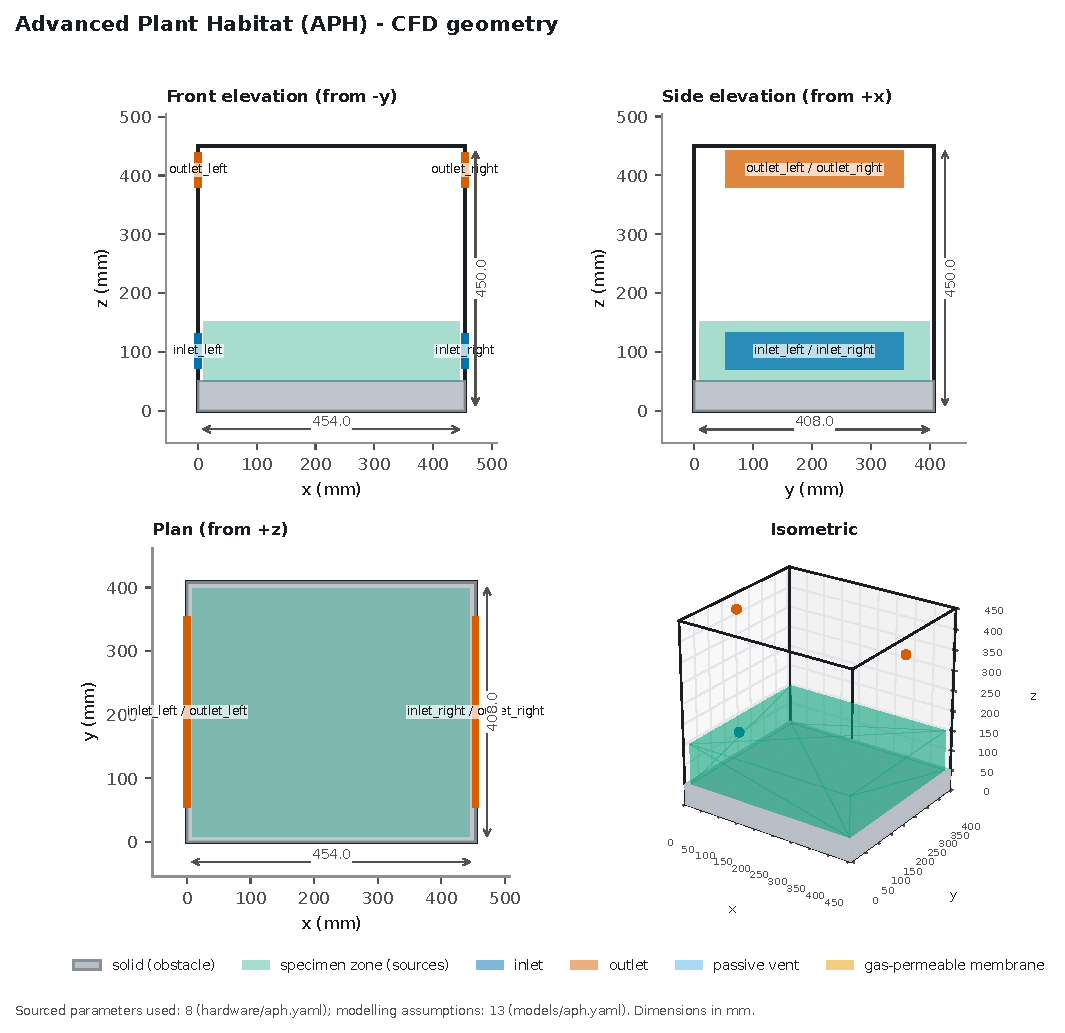
\includegraphics[width=0.78\linewidth]{../results/figures/ortho_aph.pdf}
\caption{Advanced Plant Habitat growth chamber as modelled (PH-04 set-points).}
\end{figure}
\begin{figure}[htbp]\centering
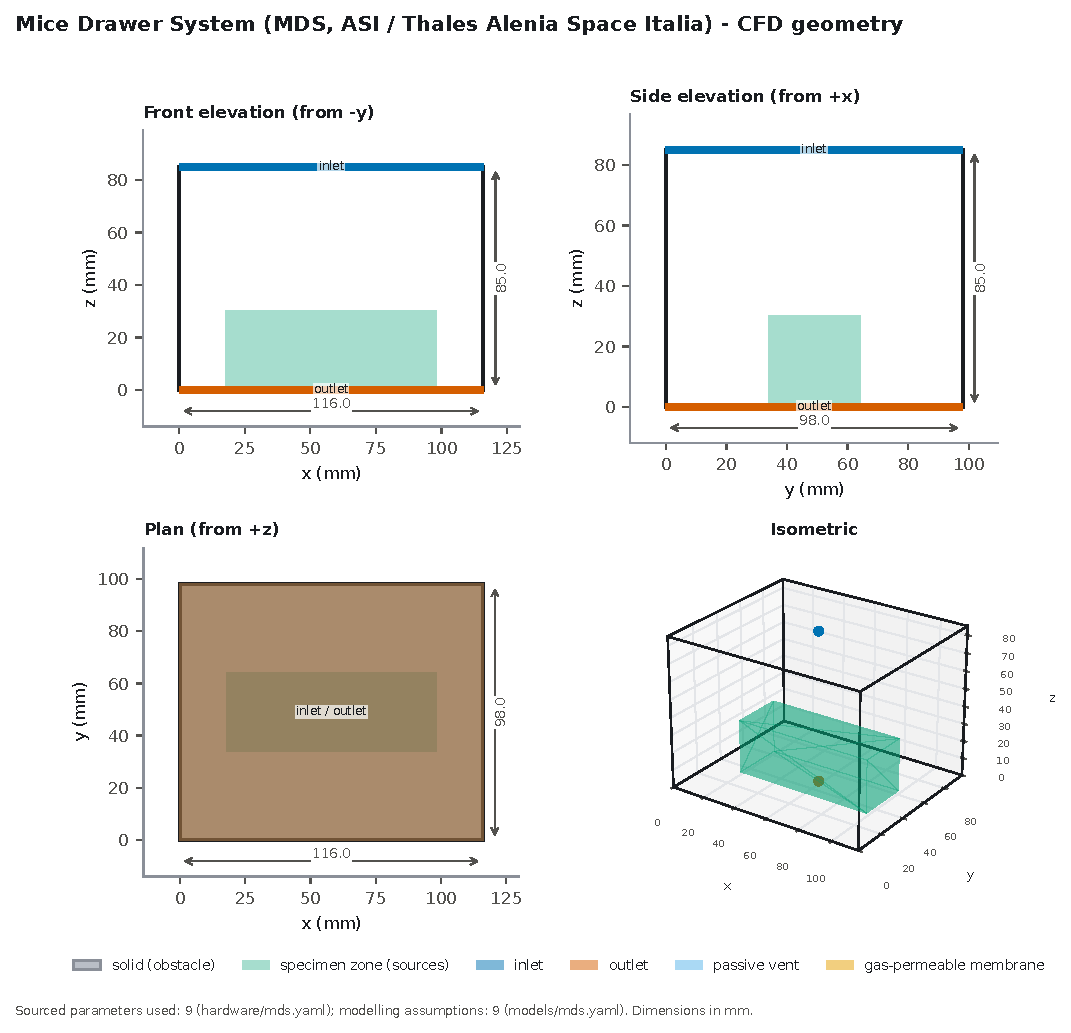
\includegraphics[width=0.78\linewidth]{../results/figures/ortho_mds.pdf}
\caption{One Mice Drawer System cage as modelled.}
\end{figure}
\begin{figure}[htbp]\centering
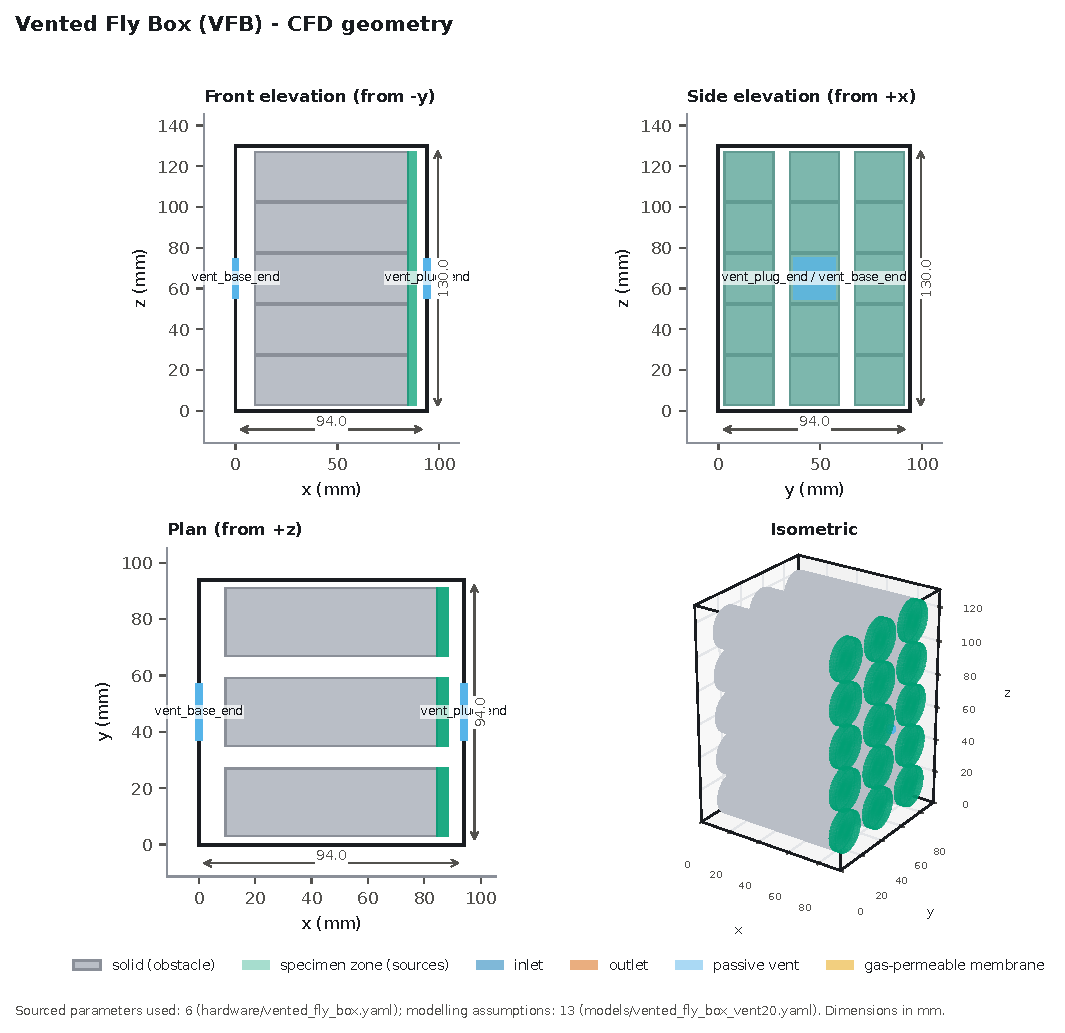
\includegraphics[width=0.78\linewidth]{../results/figures/ortho_vented_fly_box_vent20.pdf}
\caption{Vented Fly Box as modelled (20\,mm vents; the 60\,mm variant differs only in vent size).}
\end{figure}
\begin{figure}[htbp]\centering
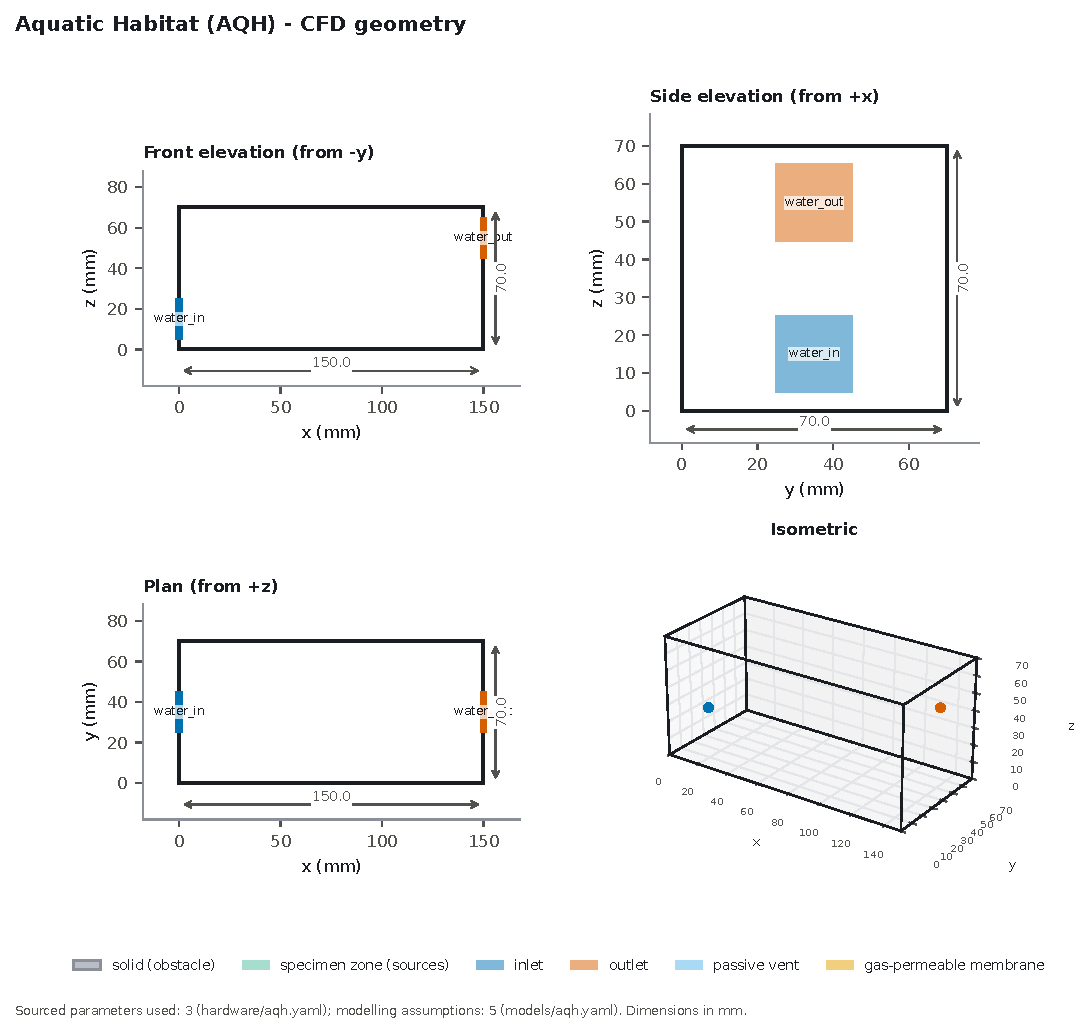
\includegraphics[width=0.78\linewidth]{../results/figures/ortho_aqh.pdf}
\caption{One Aquatic Habitat aquarium as modelled (water).}
\end{figure}

\FloatBarrier
\section*{Supplementary Note S7. Field slices}
\begin{figure}[htbp]\centering
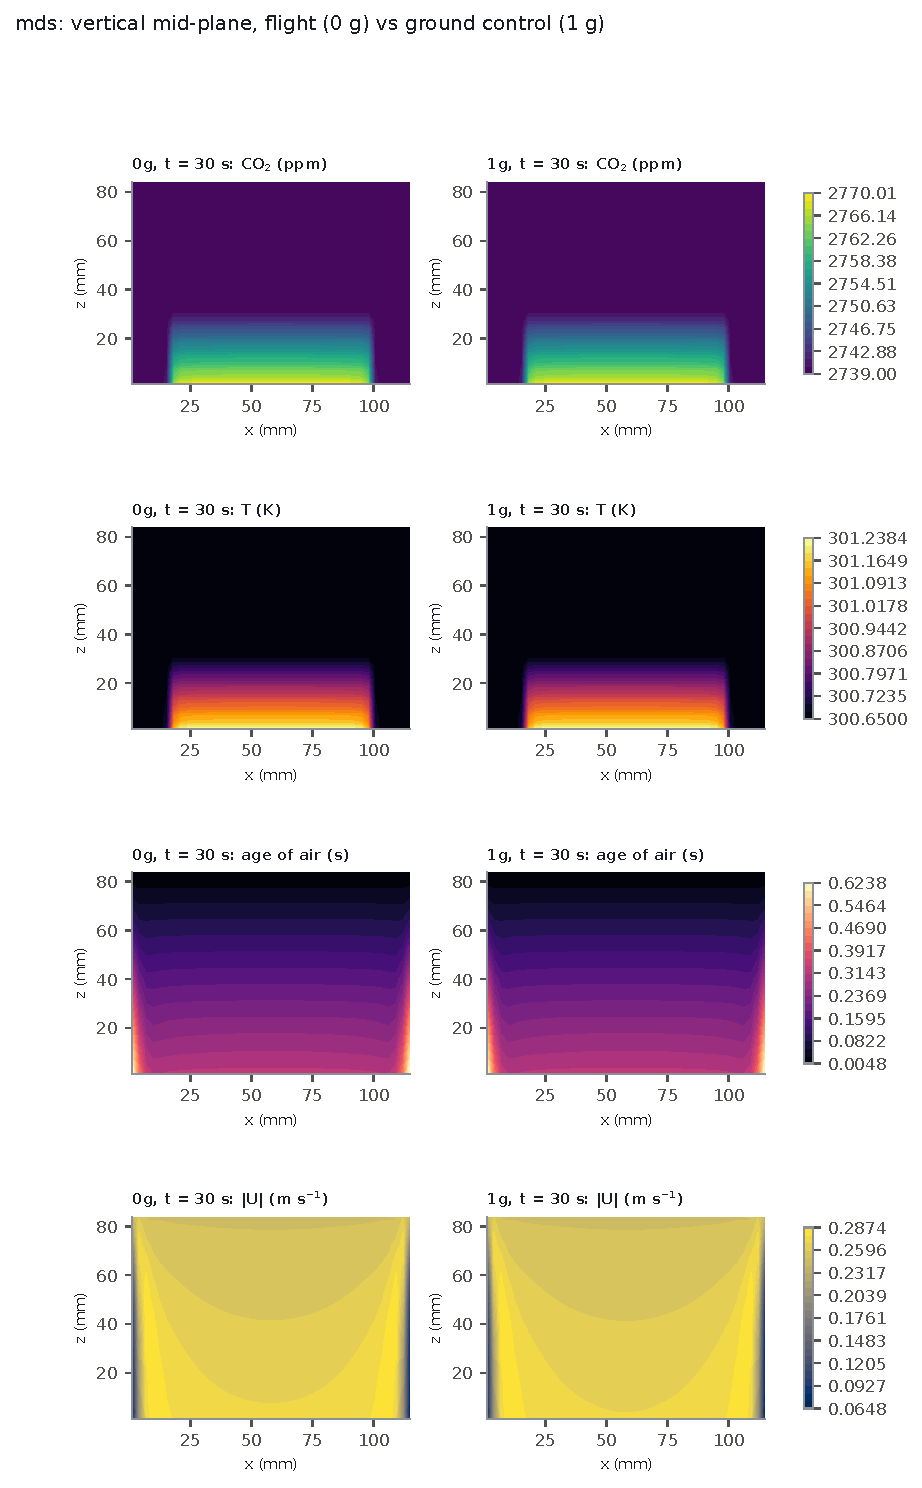
\includegraphics[width=0.8\linewidth]{../results/figures/fields_mds_medium.pdf}
\caption{MDS cage, vertical mid-plane at the end of the run, 0\,$g$ and 1\,$g$.}
\end{figure}
\begin{figure}[htbp]\centering
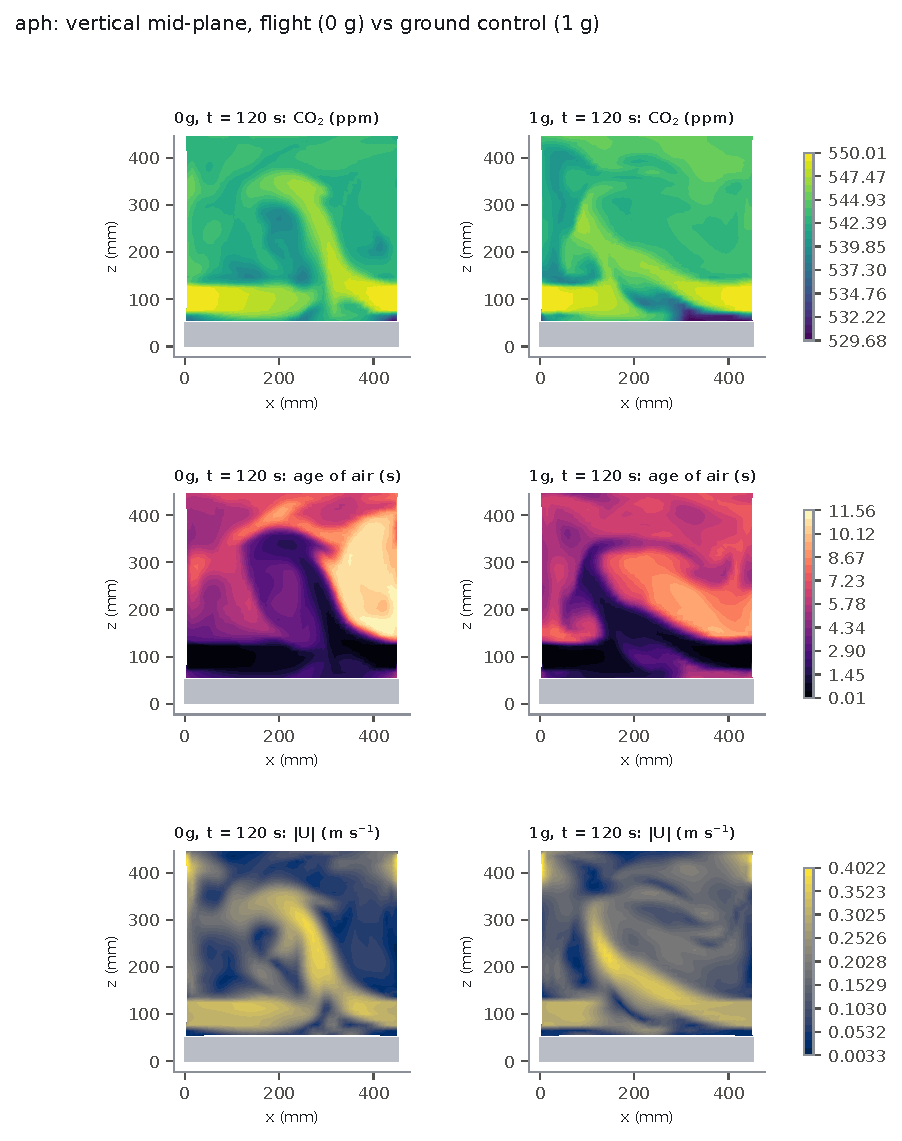
\includegraphics[width=0.8\linewidth]{../results/figures/fields_aph_medium.pdf}
\caption{APH growth chamber, vertical mid-plane at the end of the run, 0\,$g$ and 1\,$g$.}
\end{figure}
\begin{figure}[htbp]\centering
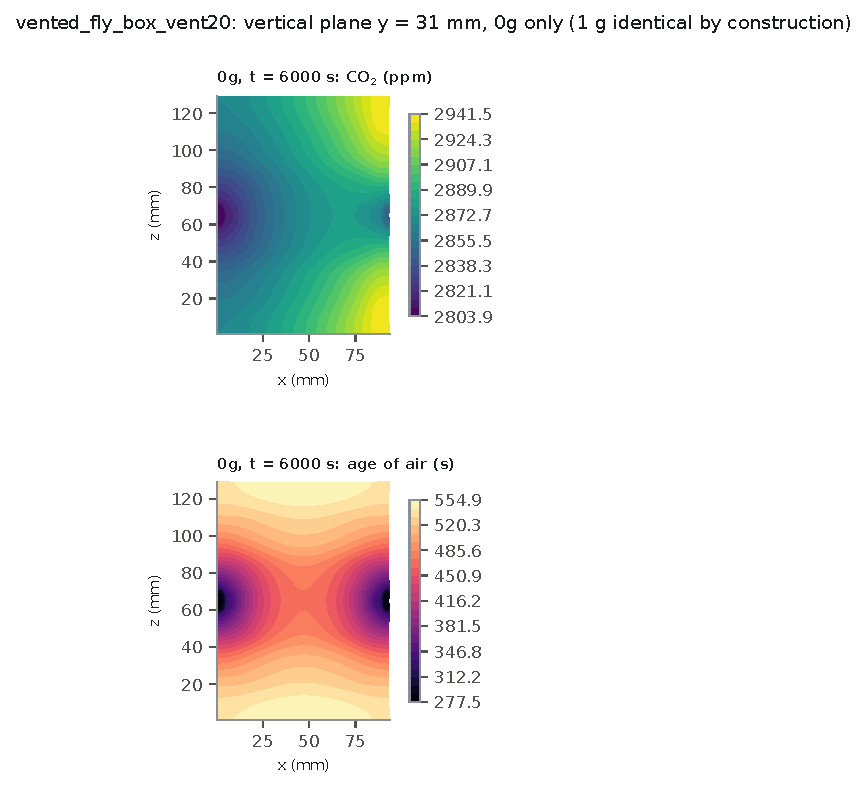
\includegraphics[width=0.8\linewidth]{../results/figures/fields_vented_fly_box_vent20_medium.pdf}
\caption{Vented Fly Box (20\,mm vents), vertical mid-plane at the end of the run, 0\,$g$ and 1\,$g$.}
\end{figure}
\begin{figure}[htbp]\centering
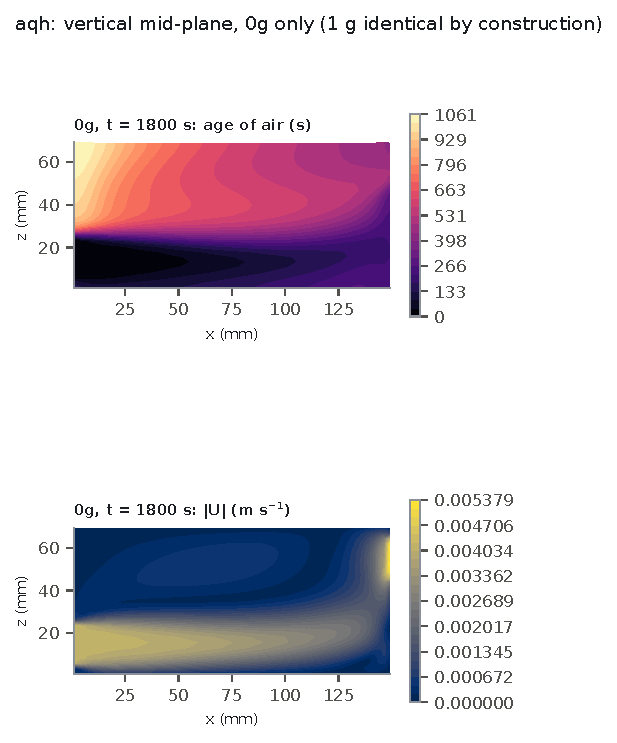
\includegraphics[width=0.8\linewidth]{../results/figures/fields_aqh_medium.pdf}
\caption{AQH aquarium, vertical mid-plane at the end of the run, 0\,$g$ and 1\,$g$.}
\end{figure}

\FloatBarrier
\section*{Supplementary Note S8. Environment cards}
Time series of specimen-zone excess over the supply or initial state, 0\,$g$ (blue) and 1\,$g$ (red), medium meshes.
\begin{figure}[htbp]\centering
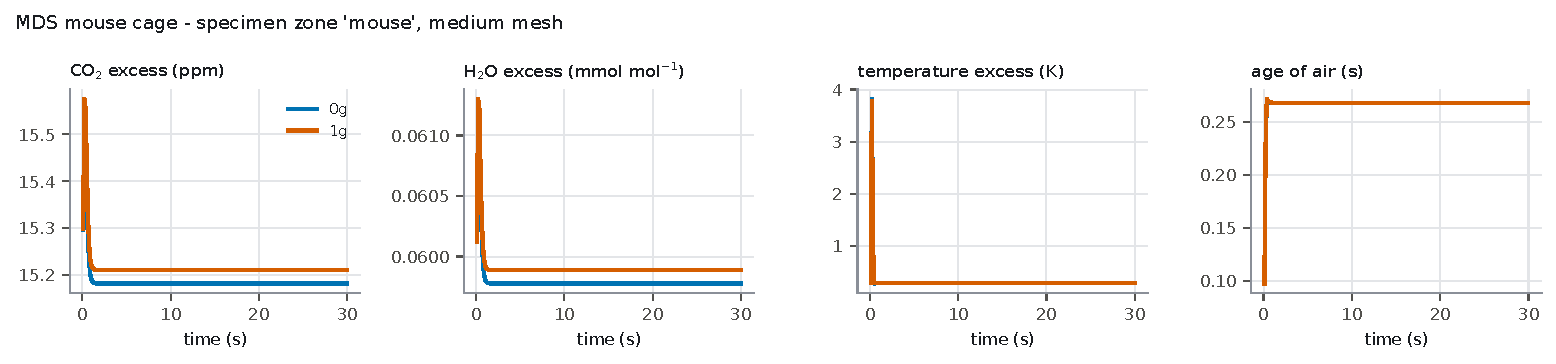
\includegraphics[width=\linewidth]{../results/figures/card_mds_medium.pdf}
\caption{MDS cage.}
\end{figure}
\begin{figure}[htbp]\centering
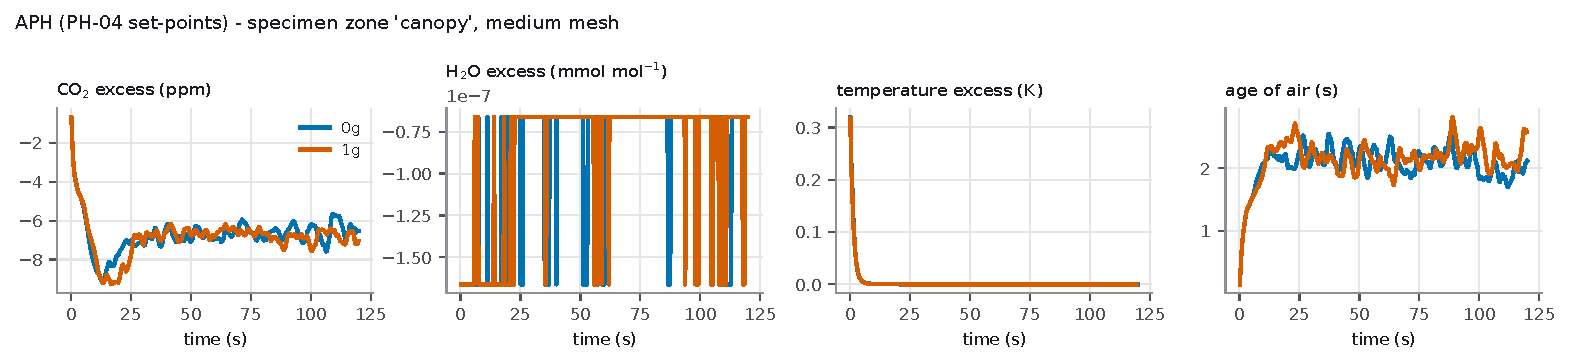
\includegraphics[width=\linewidth]{../results/figures/card_aph_medium.pdf}
\caption{APH, PH-04 set-points.}
\end{figure}
\begin{figure}[htbp]\centering
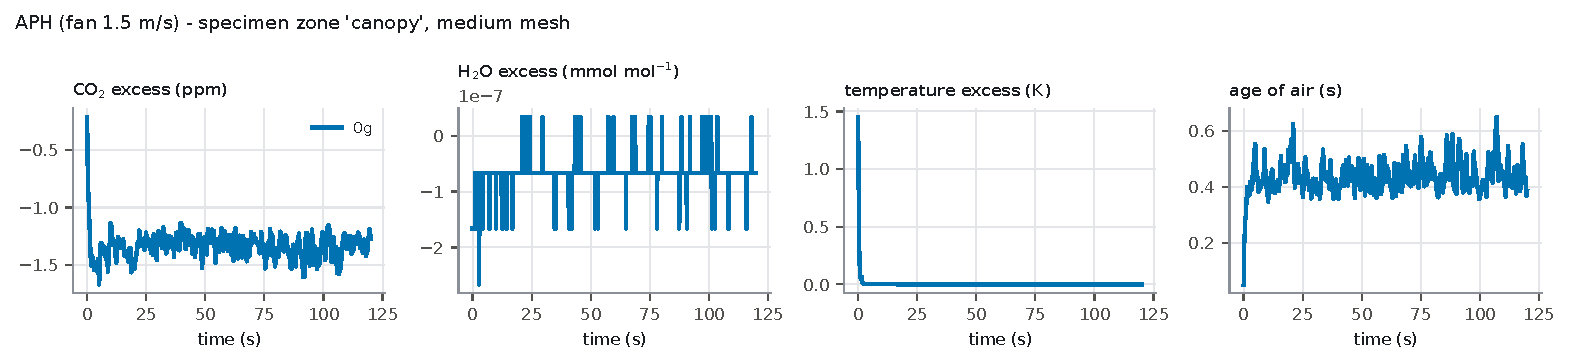
\includegraphics[width=\linewidth]{../results/figures/card_aph_fanmax_medium.pdf}
\caption{APH, fan at 1.5 m/s.}
\end{figure}
\begin{figure}[htbp]\centering
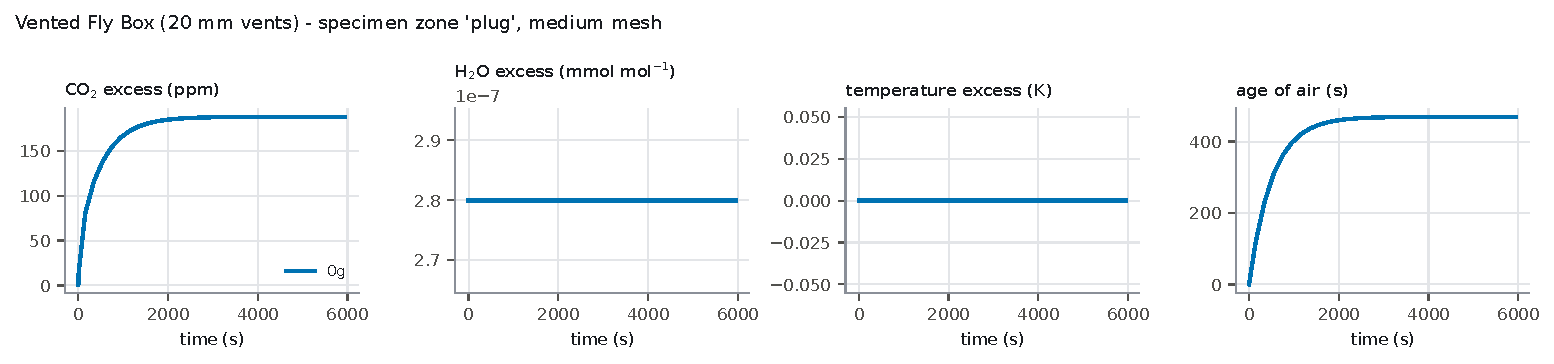
\includegraphics[width=\linewidth]{../results/figures/card_vented_fly_box_vent20_medium.pdf}
\caption{Vented Fly Box, 20 mm vents.}
\end{figure}
\begin{figure}[htbp]\centering
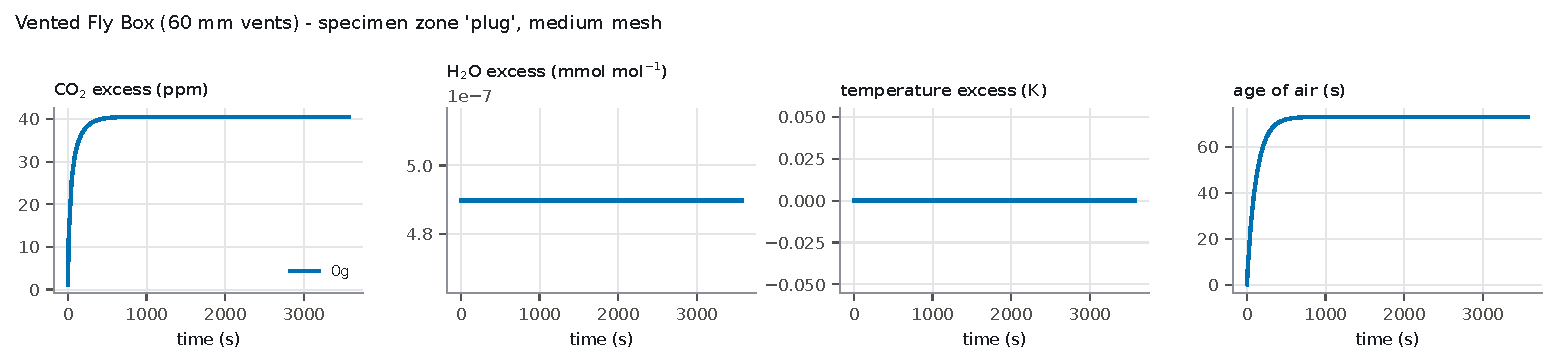
\includegraphics[width=\linewidth]{../results/figures/card_vented_fly_box_vent60_medium.pdf}
\caption{Vented Fly Box, 60 mm vents.}
\end{figure}
\begin{figure}[htbp]\centering
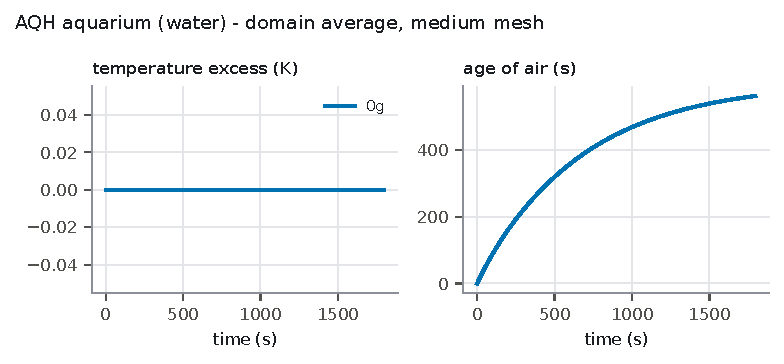
\includegraphics[width=\linewidth]{../results/figures/card_aqh_medium.pdf}
\caption{AQH aquarium (water).}
\end{figure}

\FloatBarrier
\section*{Supplementary Note S9. ISS cabin telemetry}
\textbf{Source and processing.} The telemetry and daily absorbed dose of all \hwNEdaMissions{} missions in the
OSDR Environmental Data App \citep{eda} were archived verbatim with checksums
(\nolinkurl{data/raw/2026-10-12/eda/}). The app describes them as measurements ``recorded in the ISS cabin
and ground control''. Quality control (\nolinkurl{src/hwreview/eda.py}) merges duplicated timestamps, removes
values outside physical bounds (temperature 5--40\,$^\circ$C, relative humidity 1--100\%, CO$_2$
100--20\,000\,ppm) and removes CO$_2$ values held unchanged for two hours or more, which are fills: in RR-1 the
flight series holds \hwEdaRrOneFillValue{}\,ppm for \hwEdaRrOneFillHours{}\,h from the day of launch. Each mission was
restricted to its habitation period on the ISS, chosen from the app's milestones
(\nolinkurl{data/curated/eda_mission_windows.csv}). Flight$-$ground differences use hourly means, after shifting
the ground series by the lag (within $\pm$7 days) that minimises the median absolute difference in CO$_2$, or
in temperature where CO$_2$ is absent.

\textbf{Cabin conditions for the models.} The exterior of the cabin-ventilated hardware (mouse-cage supply air,
fly-box vents) is the median of the quality-controlled RR-1 flight series over the habitation period:
\hwEdaCabinCo{}\,ppm CO$_2$, \hwEdaCabinT{}\,$^\circ$C and \hwEdaCabinRh\% relative humidity
(\nolinkurl{hardware/_iss_cabin.yaml}, \nolinkurl{results/tables/T11a_cabin_rr1.csv}). The ranges that
\citet{choi2020} report for the U.S. Lab cabin during RR-1 equal, to the last digit, the extremes of the app's
\emph{ground-control} series over the same dates (CO$_2$ \hwEdaChoiGroundCoMin--\hwEdaChoiGroundCoMax\,ppm); the
flight series spans \hwEdaChoiIssCoMin--\hwEdaChoiIssCoMax\,ppm. We use the flight series, because its minimum
is consistent with cabin CO$_2$ whereas the ground series reads room-air values before launch; which label is
correct awaits confirmation by the data provider. Because CO$_2$ and water vapour are passive scalars in the
models, this choice shifts absolute concentrations but not the specimen-zone excesses.

\textbf{Data issues.} RR-9 telemetry is dated a year after its own dose record and milestones; its
flight$-$ground differences share one clock and are kept. RR-18 has flight series only, with relative
humidity up to \hwEdaRrEighteenRhMax\% (removed). The plant missions (VEG-01, APEX-03, APEX-04) return no values
through the API, and some rodent missions return no rows.

\begin{table}[htbp]\centering\footnotesize
\caption{ISS cabin minus ground-control environment in the OSDR Environmental Data App: median and interquartile range of hourly flight $-$ ground differences after aligning the ground series by its best lag, and the mean daily absorbed dose over the window. -- : not available (RR-9: EDA dates its telemetry a year after its dose record, so the two do not overlap).}\label{tab:telemetry}
\begin{adjustbox}{max width=\linewidth}
\begin{tabular}{llrllll}
\toprule
Mission & Habitation window & Lag (h) & $\Delta T$ ($^\circ$C) & $\Delta$RH (\%) & $\Delta$CO$_2$ (ppm) & Dose (mGy\,d$^{-1}$) \\
\midrule
RR-1 & 2014-09-25 -- 2014-10-25 & 0 & 0.00 [-0.02, 0.02] & 0.0 [-0.2, 0.2] & 9 [0, 17] & 0.20 \\
RR-3 & 2016-04-12 -- 2016-05-20 & 0 & -2.00 [-2.02, -1.97] & -0.1 [-0.5, 0.2] & 6 [-1, 15] & 0.23 \\
RR-5 & 2017-06-07 -- 2017-08-02 & 0 & 0.00 [-0.02, 0.03] & 0.0 [-0.2, 0.2] & -2 [-11, 3] & -- \\
RR-6 & 2017-12-19 -- 2018-02-06 & 0 & 0.00 [-0.02, 0.02] & 0.0 [-0.2, 0.2] & -1 [-7, 4] & 0.28 \\
RR-7 & 2018-07-04 -- 2018-09-13 & 0 & 0.00 [-0.02, 0.02] & 0.3 [0.0, 0.7] & -9 [-18, -3] & 0.29 \\
RR-9 & 2018-08-18 -- 2018-09-16 & 0 & 0.00 [-0.03, 0.02] & 0.0 [-0.2, 0.2] & -2 [-8, 3] & -- \\
RR-12 & 2019-04-21 -- 2019-05-22 & 0 & 0.00 [-0.01, 0.02] & 0.0 [-0.2, 0.1] & -44 [-50, -38] & 0.36 \\
RR-19 & 2019-12-10 -- 2020-01-08 & 0 & 0.00 [-0.07, 0.04] & 0.0 [-0.6, 0.7] & -67 [-163, -34] & 0.37 \\
RR-10 & 2020-12-09 -- 2021-01-03 & 0 & 0.00 [0.00, 0.01] & 0.0 [0.0, 0.0] & -38 [-74, -17] & -- \\
RR-23 & 2020-12-09 -- 2021-01-15 & -1 & 0.00 [-0.08, 0.09] & 1.0 [0.1, 1.9] & 33 [-1, 118] & 0.35 \\
RR-18 & 2021-12-23 -- 2022-01-24 & -- & -- & -- & -- & -- \\
RR-25 & 2022-11-29 -- 2023-01-25 & 0 & 0.08 [0.03, 0.13] & -- & -- & -- \\
RR-20 & 2023-11-10 -- 2023-12-22 & 0 & -0.10 [-0.23, -0.02] & -- & -- & -- \\
RR-28 & 2024-03-24 -- 2024-04-30 & 0 & -0.06 [-0.09, -0.03] & -- & -- & -- \\
\bottomrule
\end{tabular}
\end{adjustbox}
\end{table}


\begin{figure}[htbp]\centering
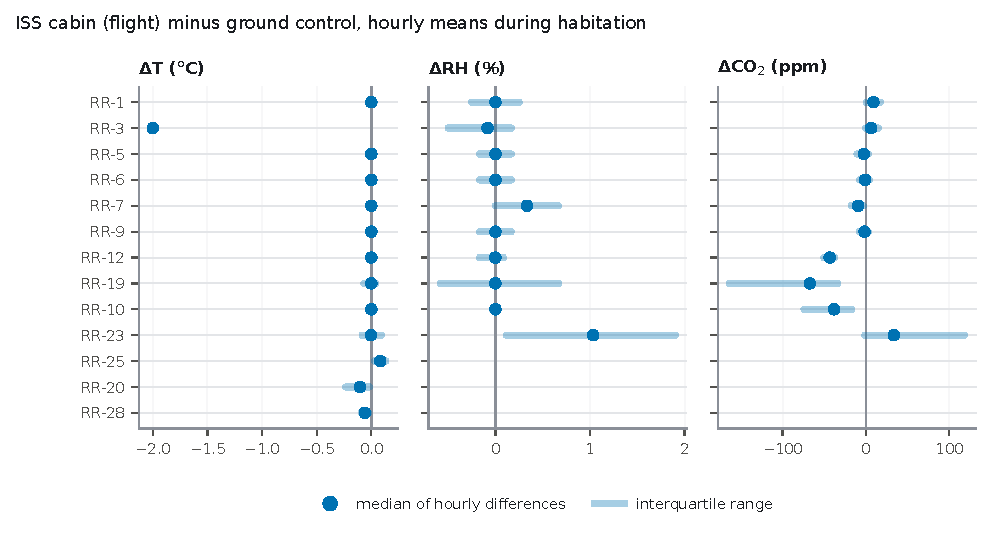
\includegraphics[width=\linewidth]{../results/figures/F9_flight_ground_offsets.pdf}
\caption{Flight (ISS cabin) minus ground-control environment for each Rodent Research mission with both series,
from the OSDR Environmental Data App: median and interquartile range of hourly differences during habitation.
Missions without relative humidity or CO$_2$ series show temperature only.}\label{fig:telemetry}
\end{figure}

\bibliographystyle{unsrtnat}
\bibliography{references}
\end{document}
